\documentclass[unicode,12pt, A4j]{ltjsarticle}% 'unicode'が必要
 %\usepackage{luatexja}% 日本語したい
 \usepackage{luatexja-fontspec}
 %\usepackage[hiragino-pron]{luatexja-preset}% IPAexフォントしたい(ipaex)
 \usepackage[hiragino-pron,deluxe,expert,bold]{luatexja-preset}

\usepackage{tikz}
\usepackage{caption}
\usepackage{subcaption}
\usetikzlibrary{calc}


% triangle (Q1)
\newcommand{\drawTriangle}[3]{
  % 三角形 #1: 左下, #2: 右下, #3: 上
  \draw (#1) -- (#2) -- (#3) -- cycle;
}

\newcommand{\recursiveTriangleQTwo}[4]{% #1, #2, #3: 座標名; #4: 深さ; #5: 識別子
  \ifnum#4=0
    \drawTriangle{#1}{#2}{#3};
  \else
    % 中点を計算して名前を付ける - 一意な識別子を使用
    \path let
      \p1 = (#1), \p2 = (#2), \p3 = (#3)
    in
      coordinate (MAB2) at ($ (\p1)!0.5!(\p2) $)
      coordinate (MBC2) at ($ (\p2)!0.5!(\p3) $)
      coordinate (MCA2) at ($ (\p3)!0.5!(\p1) $);
    \drawTriangle{#1}{#2}{#3};
    \drawTriangle{MAB2}{MBC2}{MCA2};
  \fi
}

\newcommand{\recursiveTriangleQThree}[3]{% #1, #2, #3: 座標名; #4: 深さ; #5: 識別子
    % 中点を計算して名前を付ける - 一意な識別子を使用
    \path let
      \p1 = (#1), \p2 = (#2), \p3 = (#3)
    in
      coordinate (MAB3) at ($ (\p1)!0.5!(\p2) $)
      coordinate (MBC3) at ($ (\p2)!0.5!(\p3) $)
      coordinate (MCA3) at ($ (\p3)!0.5!(\p1) $);
    \drawTriangle{#1}{#2}{#3};
    \drawTriangle{MAB3}{MBC3}{MCA3}; 
    % 呼び出し元の識別子#5に追加の識別子を付けて一意性を確保
    \recursiveTriangleQTwo{#1}{MAB3}{MCA3}{1}
    \recursiveTriangleQTwo{MAB3}{#2}{MBC3}{1}
    \recursiveTriangleQTwo{MCA3}{MBC3}{#3}{1}
}

\newcommand{\recursiveTriangleQFour}[3]{% #1, #2, #3: 座標名; #4: 深さ; #5: 識別子
    % 現在の一意な識別子を作成
    % 中点を計算して名前を付ける - 一意な識別子を使用
    \path let
      \p1 = (#1), \p2 = (#2), \p3 = (#3)
    in
      coordinate (MAB4) at ($ (\p1)!0.5!(\p2) $)
      coordinate (MBC4) at ($ (\p2)!0.5!(\p3) $)
      coordinate (MCA4) at ($ (\p3)!0.5!(\p1) $);
    \drawTriangle{#1}{#2}{#3};
    \drawTriangle{MAB4}{MBC4}{MCA4}; 
    \recursiveTriangleQThree{#1}{MAB4}{MCA4}
    \recursiveTriangleQThree{MAB4}{#2}{MBC4}
    \recursiveTriangleQThree{MCA4}{MBC4}{#3}
}


\begin{document}

\begin{figure}[h]
\centering

% Q1
\begin{subfigure}[b]{0.22\textwidth}
\centering
\begin{tikzpicture}[scale=2]
  \coordinate (A) at (0,0);
  \coordinate (B) at (1,0);
  \coordinate (C) at (0.5,{sqrt(3)/2});
  \drawTriangle{A}{B}{C};
  \node[below left] at (A) {$A_1$};
  \node[below right] at (B) {$B_1$};
  \node[above] at (C) {$C_1$};
\end{tikzpicture}
\caption{図形 \( Q_1 \)}
\end{subfigure}
\hfill
% Q2
\begin{subfigure}[b]{0.22\textwidth}
\centering
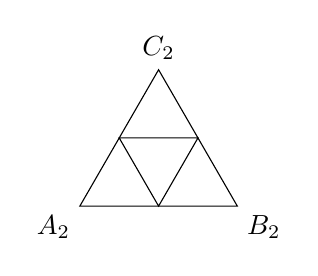
\begin{tikzpicture}[scale=2]
  \coordinate (A) at (0,0);
  \coordinate (B) at (1,0);
  \coordinate (C) at (0.5,{sqrt(3)/2});
  \recursiveTriangleQTwo{A}{B}{C}{1};
  \node[below left] at (A) {$A_2$};
  \node[below right] at (B) {$B_2$};
  \node[above] at (C) {$C_2$};
\end{tikzpicture}
\caption{図形 \( Q_2 \)}
\end{subfigure}
\hfill
% Q3
\begin{subfigure}[b]{0.22\textwidth}
\centering
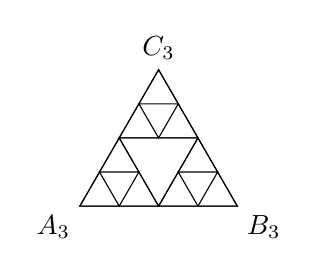
\begin{tikzpicture}[scale=2]
  \coordinate (A) at (0,0);
  \coordinate (B) at (1,0);
  \coordinate (C) at (0.5,{sqrt(3)/2});
  \recursiveTriangleQThree{A}{B}{C};
  \node[below left] at (A) {$A_3$};
  \node[below right] at (B) {$B_3$};
  \node[above] at (C) {$C_3$};
\end{tikzpicture}
\caption{図形 \( Q_3 \)}
\end{subfigure}
\hfill
% Q4
\begin{subfigure}[b]{0.28\textwidth}
\centering
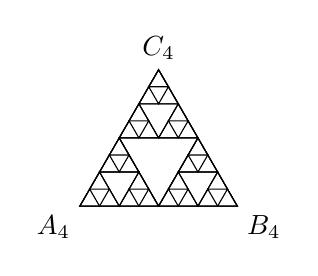
\begin{tikzpicture}[scale=2]
  \coordinate (A) at (0,0);
  \coordinate (B) at (1,0);
  \coordinate (C) at (0.5,{sqrt(3)/2});
  \recursiveTriangleQFour{A}{B}{C};
  \node[below left] at (A) {$A_4$};
  \node[below right] at (B) {$B_4$};
  \node[above] at (C) {$C_4$};
\end{tikzpicture}
\caption{図形 \( Q_4 \)}
\end{subfigure}

% \caption{再帰的に構成される三角形 \( Q_n \)}
\end{figure}

\end{document}
